\begin{figure}[h!]
	\centering
\begin{minipage}{\textwidth}\centering
\mybox{
\begin{tabular}{cc|cc}
\multicolumn{2}{c}{\textbf{HOMO}} & \multicolumn{2}{c}{\textbf{LUMO}} \\
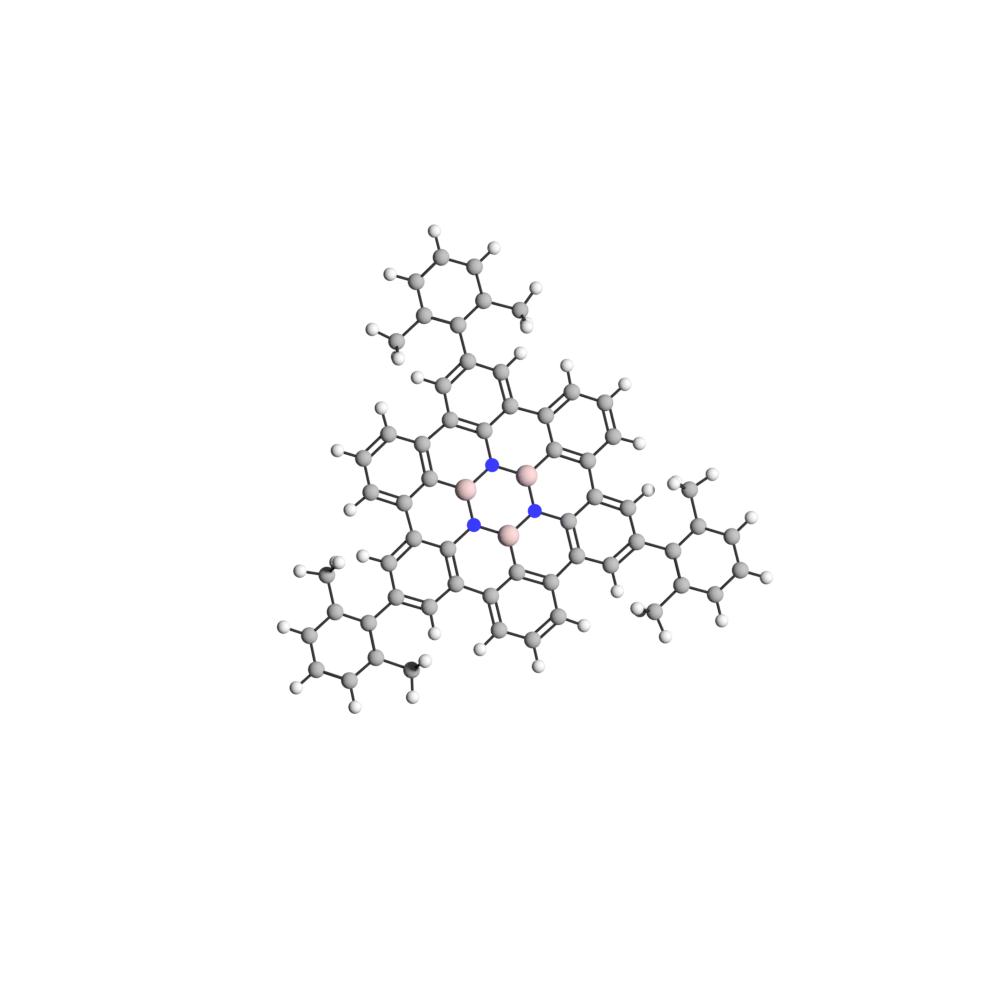
\includegraphics[width=2.7cm]{./images/molecules/HBBNC-flat} & 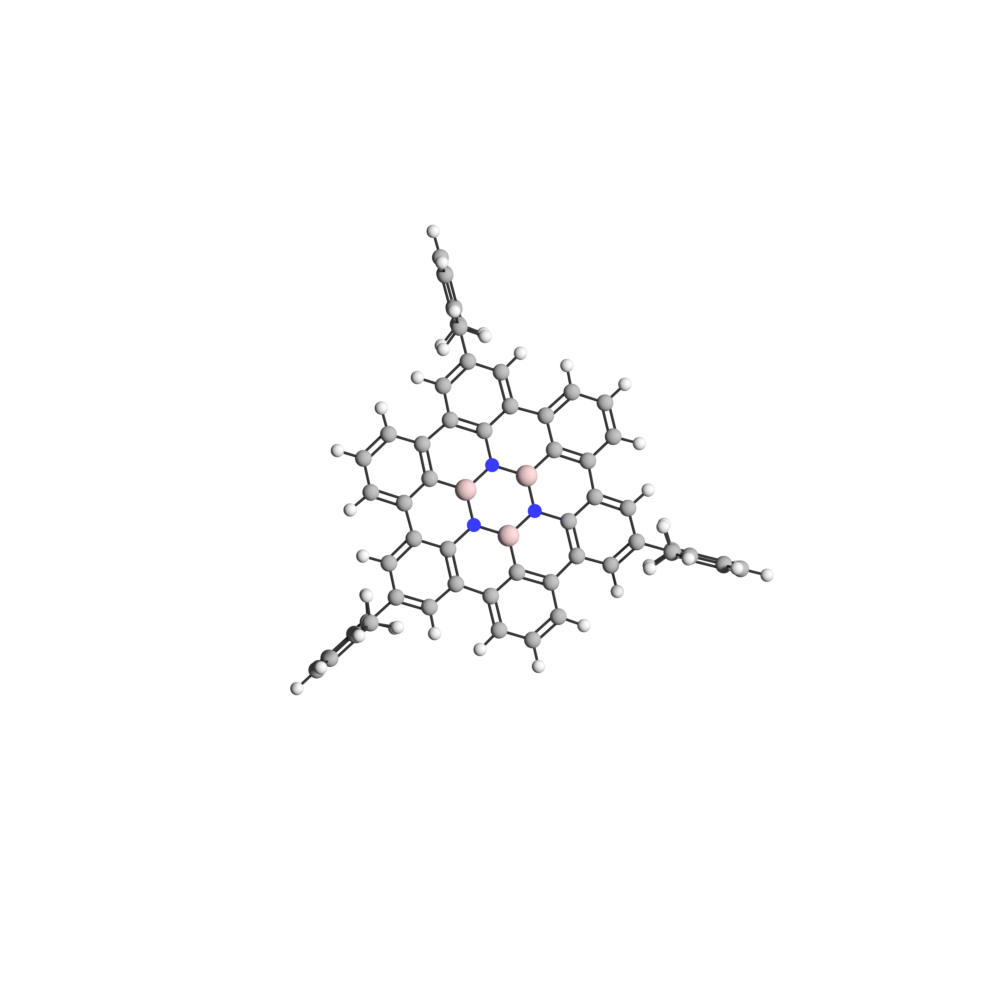
\includegraphics[width=2.7cm]{./images/molecules/HBBNC} & 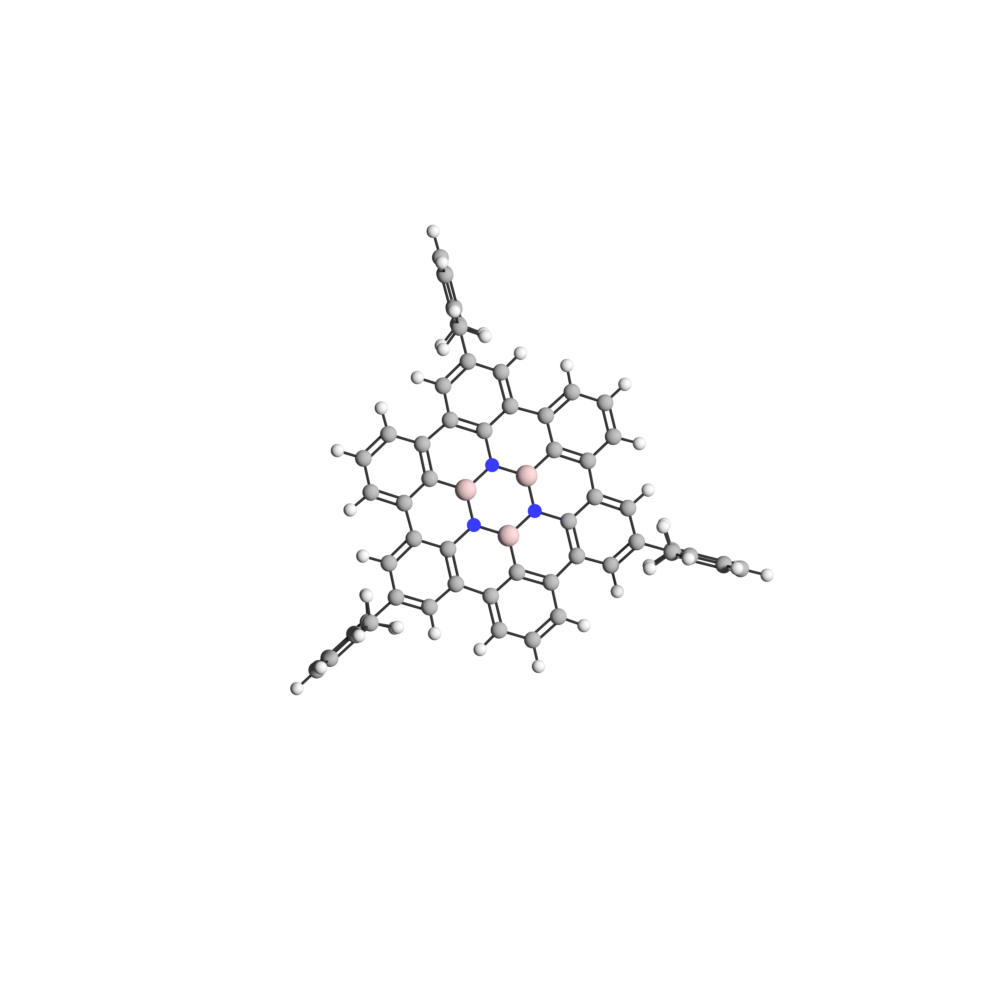
\includegraphics[width=2.7cm]{./images/molecules/HBBNC} & 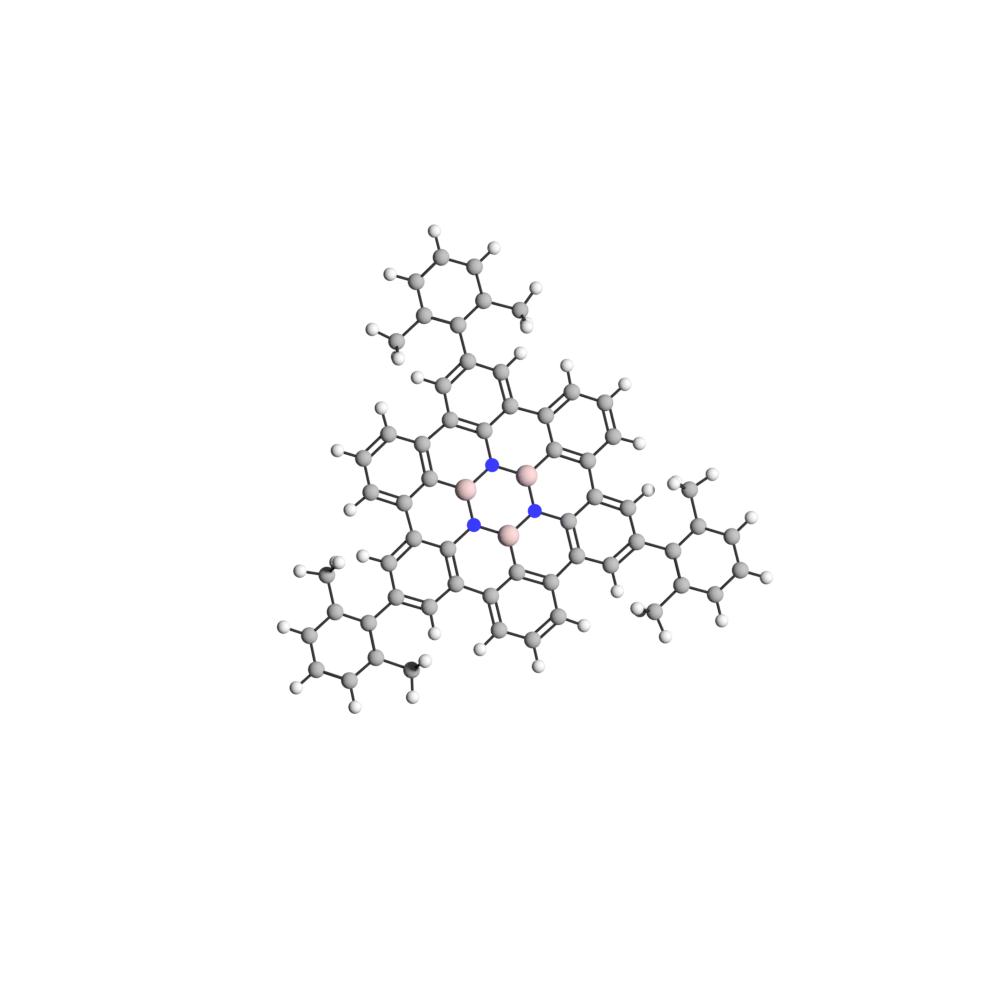
\includegraphics[width=2.7cm]{./images/molecules/HBBNC-flat} \\
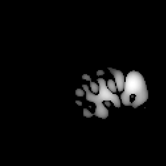
\includegraphics[width=2.7cm]{./images/molecules/orbitals/hbbnc/Flat/HOMO/153} & 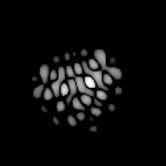
\includegraphics[width=2.7cm]{./images/molecules/orbitals/hbbnc/B3LYP/HOMO/153} &  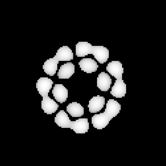
\includegraphics[width=2.7cm]{./images/molecules/orbitals/hbbnc/B3LYP/LUMO/154} &

\includegraphics[width=2.7cm]{./images/molecules/orbitals/hbbnc/Flat/LUMO/154} \\
\end{tabular}
}
\end{minipage}
\graphicspath{{./images/molecules/orbitals/hbbnc/}}
	\subfigure[]{
		\frame{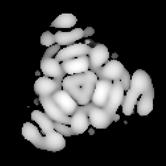
\includegraphics[width=2.7cm]{./Flat/HOMO/153-148}}
	}
	\subfigure[]{
		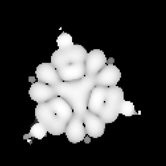
\includegraphics[width=2.7cm]{./B3LYP/HOMO/153-148}
	}
	\subfigure[]{
		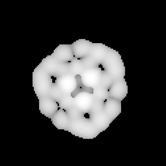
\includegraphics[width=2.7cm]{./B3LYP/LUMO/154-159}
	}
	\subfigure[]{
		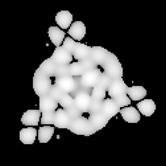
\includegraphics[width=2.7cm]{./Flat/LUMO/154-159}
	}
	%%%%%%%%%%%%%%%%%%%%%%%%%%%%%%%%%%%%%%%%%
	\subfigure[]{
		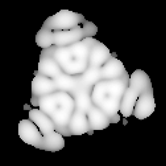
\includegraphics[width=2.7cm]{./Flat/HOMO/153-142}
	}
	\subfigure[]{
		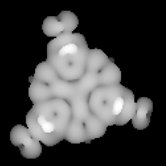
\includegraphics[width=2.7cm]{./B3LYP/HOMO/153-142}
	}
	\subfigure[]{
		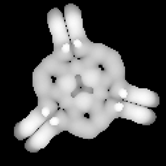
\includegraphics[width=2.7cm]{./B3LYP/LUMO/154-165}
	}
	\subfigure[]{
		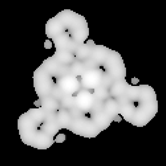
\includegraphics[width=2.7cm]{./Flat/LUMO/154-165}
	}
	%%%%%%%%%%%%%%%%%%%%%%%%%%%%%%%%%%%%%%%%%
	\subfigure[]{
		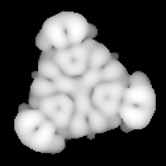
\includegraphics[width=2.7cm]{./Flat/HOMO/153-136}
	}
	\subfigure[]{
		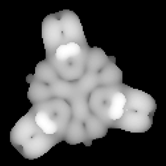
\includegraphics[width=2.7cm]{./B3LYP/HOMO/153-136}
	}
	\subfigure[]{
		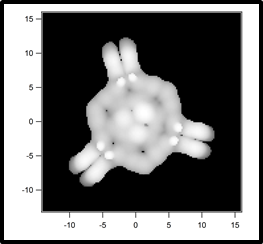
\includegraphics[width=2.7cm]{./B3LYP/LUMO/154-171}
	}
	\subfigure[]{
		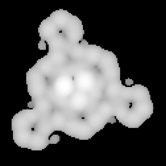
\includegraphics[width=2.7cm]{./Flat/LUMO/154-171}
	}
	%%%%%%%%%%%%%%%%%%%%%%%%%%%%%%%%%%%%%%%%%
	\subfigure[]{
		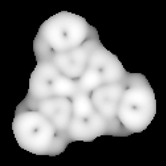
\includegraphics[width=2.7cm]{./Flat/HOMO/153-130}
	}
	\subfigure[]{
		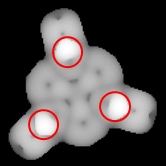
\includegraphics[width=2.7cm]{./B3LYP/HOMO/153-130-mod}
	}
	\subfigure[]{
		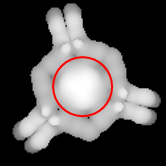
\includegraphics[width=2.7cm]{./B3LYP/LUMO/154-177-mod}
	}
	\subfigure[]{
		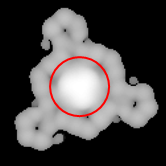
\includegraphics[width=2.7cm]{./Flat/LUMO/154-177-mod}
	}
	\caption{Integrated EHT calculated molecular orbitals for two leg configurations of HBBNC. Inner two columns show molecular configuration as predicted by a B3LYP structure optimization. Here the coronene center is parallel to the image plane while the legs are oriented with \SI{90}{\degree} rotation. Outer columns show the molecule with rotated di-methyl functionalization to lie in the image plane. The difference in shape at the leg funtionalization is best visible for occupied states as opposed to unoccupied states where similar features develop at the center. Images are \SI{2.5}{\nano \meter} wide.}
\label{fig:HBBNC-EHT-leg-configuration}
\end{figure}
\vfill